\chapter{Added Components}
\label{chapter:4}
\section{SimBaD-Client}
From user perspective, the \textit{SimBaD-Client} is the central point of the application. First section will discuss the technology and design patters used.The second section will talk about the two main application views- the configuration editor and the simulation pipeline view. Finally, the way of serving application will be discussed and what will be placed in docker container responsible for \textit{SimBaD-Client}.
\subsection{Technology}
\subsubsection{Overview of frameworks}
The web development ecosystem in current year is as rich as it is complicated. For anything other than a simple static website, many tools are necessary to solve problems such as making the website work in different browsers, internationalization, or production and development builds. There are numerous frontend JavaScript frameworks, such as Angular, React or Vue to name a few. One can achieve exactly the same result using those frameworks, so the choice between mainly comes down to developer preference. For the \textit{SimBaD-Client}, Angular is the framework of choice, due to its excellent support for \textit{Typescript}, building and configuration with \textit{Angular-CLI}, \textit{Angular Matrial UI} library and \textit{Swagger Codegen} support, used to generate client libraries communicating with \textit{SPS} \cite{SwaggerCodegen}.
\subsubsection{Monorepo pattern}
The project was bootstrapped with\textit{Angular-CLI} and \textit{Nx} using monorepo pattern \cite{NxCLI}. Monorepo, is a pattern that helps organize and share code between multiple \textit{JavaScript} applications. Code in monorepo, as the name indicates is put in single repository. Monorepo ensures that everything at a single commit works together - for code in separate repositories, the state of application is a combination of several commits from each repository. Another benefit, especially important for frontend applications, is that it allows to centralize the build system and and toolchain - all of the code in monorepo is build using Angular-CLI and depends on the same packages. It makes easy to split the code into libraries, and to compose applications using those libraries. For \textit{SimBaD-Client} it allows to split the client code into apps, such as \textit{SimBaD-Client} app, developer server for building frontend independently from backend, and shared \textit{API} and \textit{UI} libraries. The \textit{CI} process is also simplified, as each change and applications and libraries that are affected by this change can be tested, and pass for such tests proves that each application in monorepo works as indented \cite{MonorepoSavkin}.
\subsubsection{Reactive programming and store architecture}
Reactive programming is a programming paradigm that deals with asynchronous data streams - sequences of some kind of events ordered in time. Data streams can be created from anything, for example, from click events, \textit{HTTP} calls to user inputs or variable declarations. Those streams can then be manipulated in multiple ways, for example they can be filtered, merged or mapped to other streams \cite{RxJSOperators}. Streams can also be "subscribed to" or "consumed" to produce some kind of side effect, like showing notification in \textit{UI}, when some \textit{API} returns specific status \cite{RxJSSub}. Reactive programming changes the way that application components communicate with each other. Instead of pushing data directly into components, or components asking explicitly for data, in reactive programming they automatically "react" to data changes. The most popular library for reactive programming is \textit{Rx}, and \textit{RxJS} is the \textit{JavaScript} version of this library \cite{RxJSSource}. For web applications, where lots of code is executed asynchronously, and there is multitude of \textit{UI} or data related events to react to, \textit{RxJS} allows to write code that handles that in a maintainable and concise way.
\begin{figure}[h!]
	\centering
		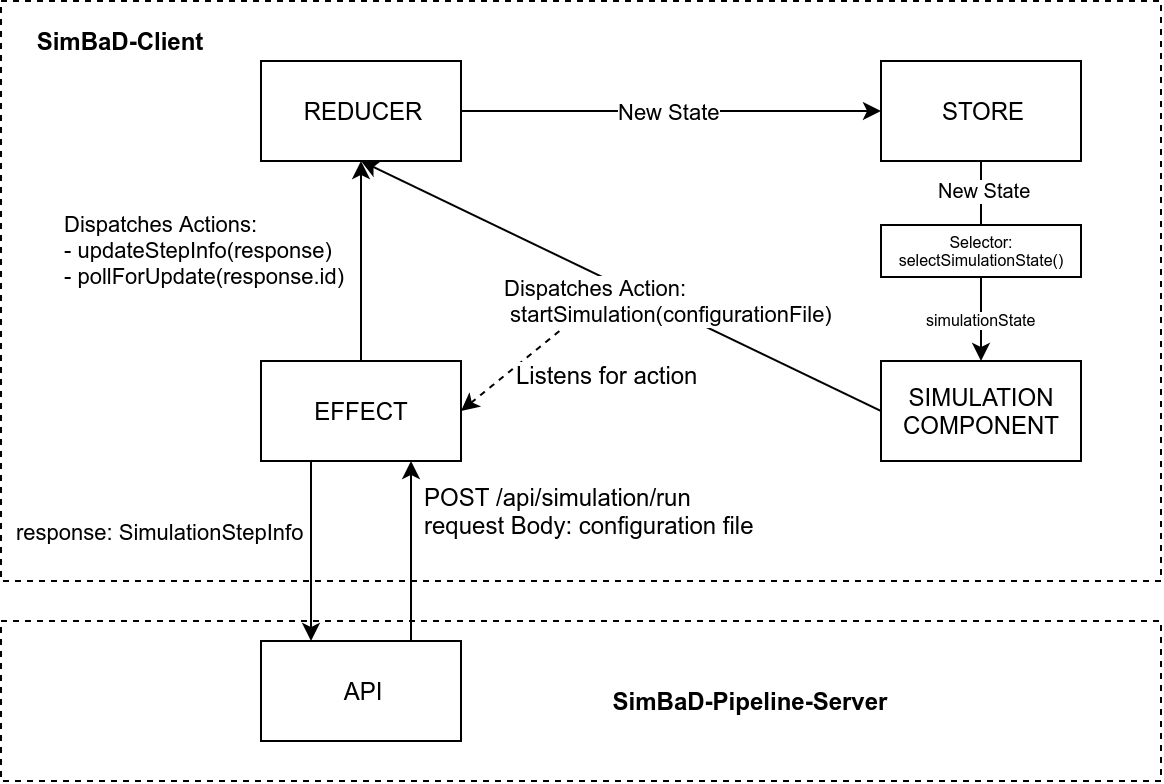
\includegraphics[width=0.9\linewidth]{diagrams/ngrx.png}
	\caption{Example of \textit{NgRX} flow in \textit{SimBaD-Client}}
	\label{fig:ngrx}
\end{figure}
Reactive programming works very well with store architecture. The store can be thought of as a client-side database, where all data needed by application resides. The store reflects the complete state of application, and all of the components of application treat the store as a single source of truth. The main problem that the store architecture solves, is the problem of passing data between  components \cite{AngularUniWhyStore}.
In \textit{Angular}, data can be passed between components in server ways - from parent to child using t\textit{Input()} member variables, from child to parent using \textit{EventEmmiters()} and between unrelated components using services \cite{AngularPassingData}. Problems arise when data needs to be passed several levels down in component tree - the root component has the data, and the leaf components needs this data, however for the component nodes along the way, that do not need the data, extraneous Input properties must be added. Store architecture bypasses that problem, by providing single source of truth or the store for all of the components to get data from and push data to. When actor such as user or server changes some data, this change is pushed to store, and automatically reflected in all of the components.
\textit{NgRx} is a library that implements the store pattern, geared towards \textit{Angular} applications \cite{NgrxDocs}. \textit{NgRx} is tightly coupled with the \textit{RxJS} library, as the store itself is an observable and components need to subscribe to the store observable to get the data.
\textit{NgRx} consists of several building blocks - actions, reducers, effects and selectors \cite{NgRxStoreDocs}. The components can alter state of application or by dispatching actions to store. Actions consists of type - unique action identifier and payload - the data that is needed to change the state. Reducer is a pure function that accepts two arguments - current state of application and action. Reducer analyzes the action and returns new state that is a combination of previous state and action payload. Side effect can be something like making a http call, or showing a notification. The effects trigger when specific action is dispatched to store, and can be used to trigger side-effect based on those actions. Effects can also dispatch another action to the store, for example they can push response received from http call. Single effect can be triggered by multiple action, can dispatch multiple actions and single action can trigger multiple effects. The store can be quite big object and often, components need only a part of it. Components can subscribe to parts of the store using Selectors. In the figure \ref{fig:ngrx}, example \textit{NgRx} flow triggered by user starting the simulation is shown.

The user action, for example clicking a button, causes the component responsible for simulation view to dispatch \textit{startSimulation()} action with simulation configuration file as its payload. This triggers two separate \textit{NgRx} flows. In the first one, the action is passed to the reducer, and new state with added information that simulation has started is generated. Then the store observable emits new data and component receives a slice of this data, based on selector. The second flow starts with effect, that reacts to \textit{startSimulation()} action being dispatched. This effect makes then it \textit{POST} request to \textit{SPS} to start simulation, and receives the information about the first simulation step. Effect then dispatches two actions with response as a payload, one to update information about current information of simulation step in store, and one to start polling for step information changes. Those actions then are handled by reduce which modifies store state, and this new store state is emitted and passed to component. If dispatched actions trigger any effects, another flow starts.
\subsection{Configuration editor view}
To start simulation process user needs to pass simulation configuration file or \textit{SCF}. This file has tree-like structure and contains various objects and parameters that control the simulation process. Although those objects need have predefined value types, ranges, or enums, the exact definitions did not exists, and had to be created. Detailed description of this file and how to add new parameters to simulation can be found in appendix \ref{appendix:A}.
\begin{figure}[h!]
	\centering
		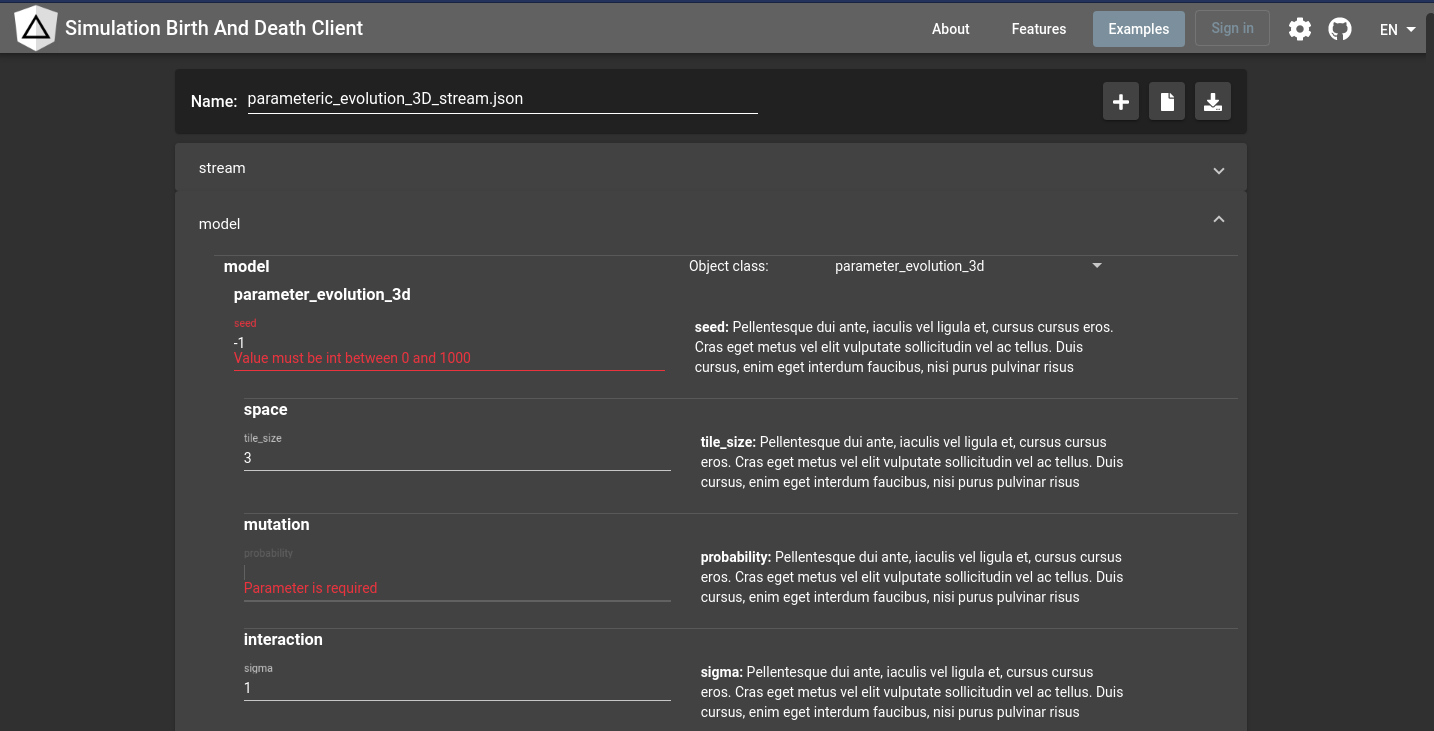
\includegraphics[width=0.9\linewidth]{screens/conf-view.png}
	\caption{The configuration editor view}
	\label{fig:conf-view}
\end{figure}
To enable user to generate valid \textit{SCF}, configuration editor was created. Configuration editor generates forms that validate the parameter values entered by user against their definitions. The form has tree structure that maps to configuration. Additionally, each form input associated with parameter displays validation messages, and parameter description. The form is generated dynamically, and adding or changing definition in object definition does not break the form, though it requires to rebuild application. The user can create new configuration, and download and upload the configuration from \textit{JSON} file. The SimBaD-CLI supports two file formats: \textit{JSON} and \textit{.simbad} which is an alias to default\textit{Boost.PropertyTree} format, but the configuration editor handels only the \textit{JSON} format. As the changes in configuration are dispatched to store, the configuration can be shared between different components. 
\begin{figure}[h!]
	\centering
		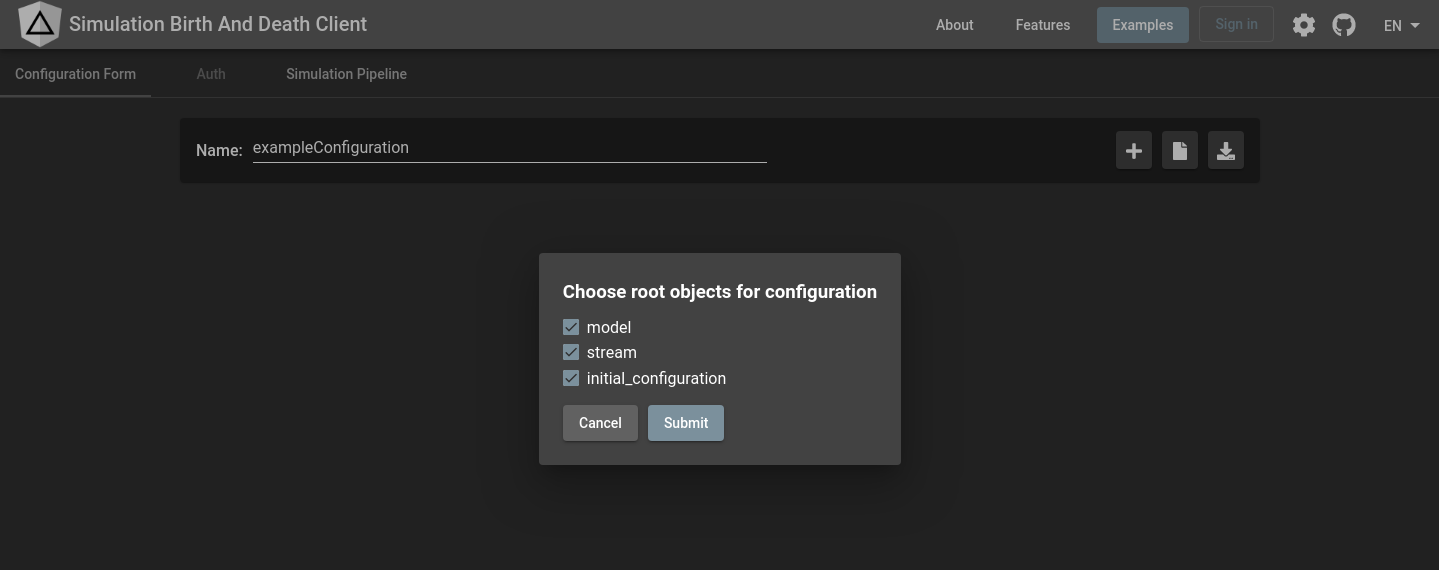
\includegraphics[width=0.9\linewidth]{screens/configuration-view-modal.png}
	\caption{Creating new configuration}
	\label{fig:conf-view-new}
\end{figure}
\subsection{Simulation pipeline view}
The second view of the application is the view that allows to monitor the simulation process. User can start simulation pipeline using this view. To start it, user can upload \textit{SCF}, or when present in store, use the previously edited \textit{SCF}. Additionally, user is able to load the results of last simulation. Each major change in step such as finishing or starting a step is accompanied by proper notification.
The simulation pipeline view consists of 3 main components, each responsible for different simulation step. Each of those components allows to view the current simulation status with information such as current step runtime status, the context of a step, and when step finishes, the resulting output files (also called simulation artifacts). Each artifact can be downloaded in \textit{.zip} format, and for images, it can also be displayed. For the SimBaD-CLI view, visible in the figure \ref{fig:sp-cli}, additional metrics regarding the process executing the simulation are displayed - the CPU usage and \textit{RAM} usage. 
\begin{figure}[h!]
	\centering
		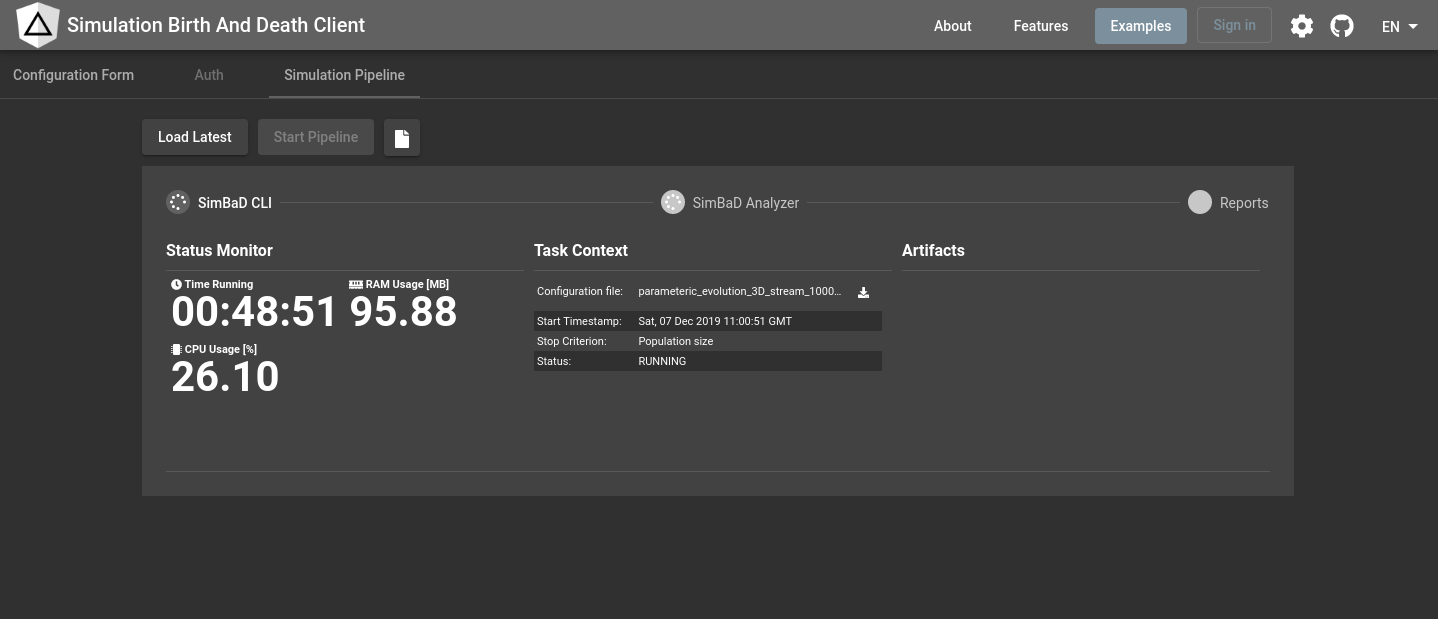
\includegraphics[width=0.9\linewidth]{screens/cli-view.png}
	\caption{Simulation pipeline view: CLI step}
	\label{fig:sp-cli}
\end{figure}
For the analyzer-view, there's a link to the \textit{Spark UI} dashboard and progress bar that displays information about total progress of analyzer job, based on already created artifacts. This view can be seen on the figure \ref{fig:sp-analyzer}.
\begin{figure}[h!]
	\centering
		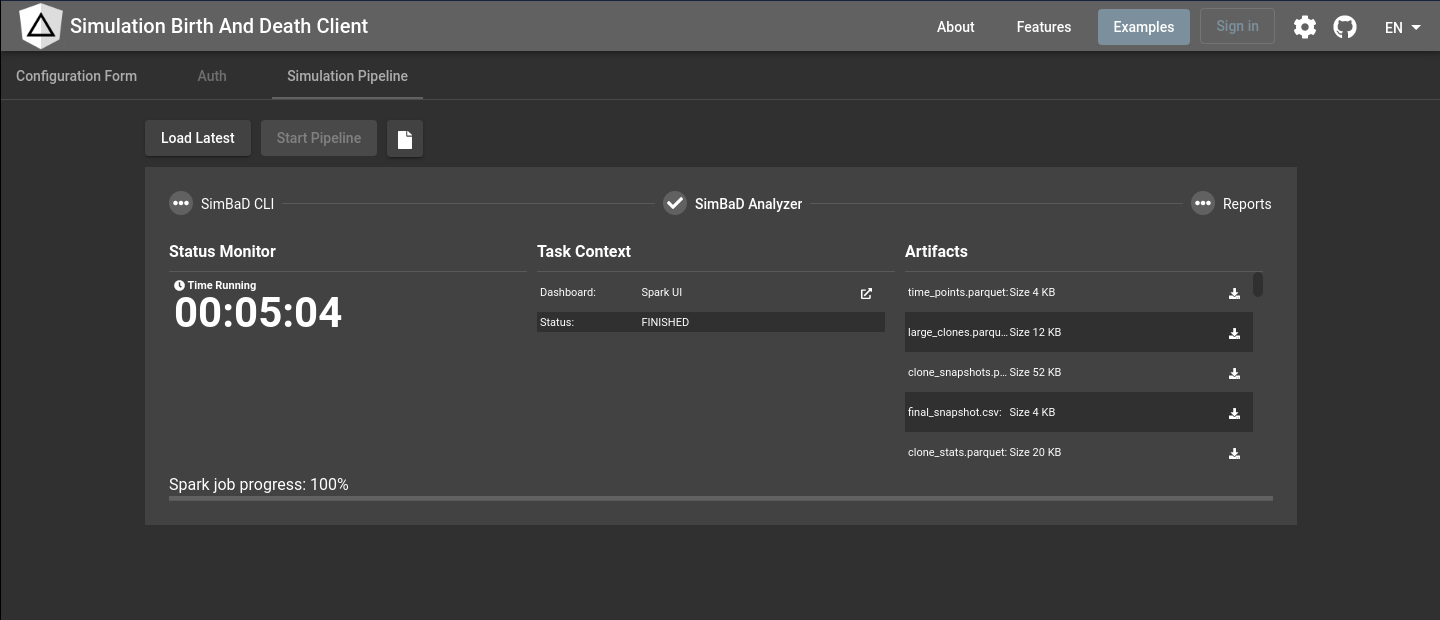
\includegraphics[width=0.9\linewidth]{screens/analyzer-view.png}
	\caption{Simulation pipeline view: Analyzer step}
	\label{fig:sp-analyzer}
\end{figure}
Finally the last step of this view is the report step. Apart from option to download the resulting plots, the user has also option to display the plots in browser. Example display of such plot is shown on the figure \ref{fig:sp-report-muller}.
\begin{figure}[h!]
	\centering
		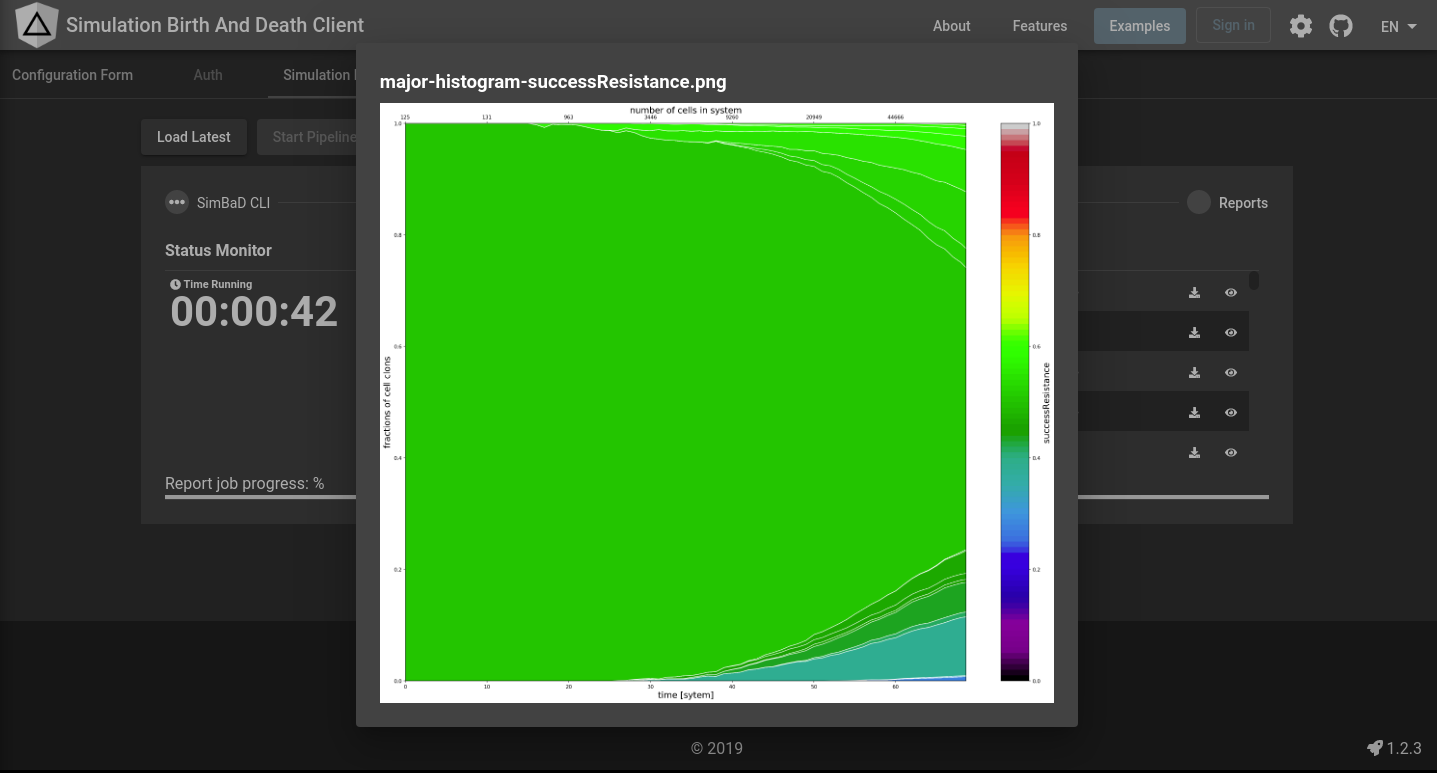
\includegraphics[width=0.9\linewidth]{screens/report-view-muller.png}
	\caption{Report view: mullerplot}
	\label{fig:sp-report-muller}
\end{figure}
\newpage
\subsection{Serving the client}
To server application from docker container first it is necessary to build it. The application can be build in two ways- the development build and the production build. The development build contains non minified code with sourcemaps that is suitable for debugging.  Minification is a process of removing redundant data from the code (such as whitespace, comments or verbose function and variable names). and sourcemaps are files that map compressed and transpiled JavaScript code to its original source files. Such build should not be server to the user, as it not optimized in size, and contains information valuable only to developer. The production on the other hand, reduces the size of the bundle applying minification tree shaking and other techniques. Such build is suitable to be actual served to user but needs an actual server to host it. There are many http servers, but for the purpose of this application the \textit{Nginx} was used. Apart from serving the files, the \textit{Nginx} also is used as reverse proxy to \textit{SPS}. 
There are two steps to create docker image for this component. First, all of the \textit{NPM} packages necesary to build the application must be installed, and after building it, the resulting files must be copied to the \textit{ /usr/share/nginx} folder. To avoid increasing the image size the docker multi-stage builds feature was used. The \textit{Dockerfile} for this component is visible on the listing \ref{list:sc-docker}.
\begin{lstlisting}[label=list:sc-docker,caption=Dockerfile used to build \textit{SimBaD-Client}, basicstyle=\footnotesize\ttfamily]
FROM node:11.1.0 as npm_builder
COPY ./package.json /usr/simbad-client/app/package.json
COPY ./package-lock.json /usr/src/app/package-lock.json

WORKDIR /usr/simbad-client/app
RUN npm install --silent

FROM npm_builder as builder
COPY . /app
ENV PATH /app/node_modules/.bin:$PATH
WORKDIR /app
RUN npm run build

FROM nginx
COPY --from=builder /app/dist/projects/simbad-client /usr/share/nginx/html
\end{lstlisting}
Dockerfile is split into three stages, the first \textit{npm\_builder} extends the community image with installed \textit{NPM} and \textit{Node}.
The \textit{package.json} files containing client dependencies are copied onto the file and the packages from this file are installed. The second stage is builder, used to generate production build. The last stage is \textit{Nginx}. It starts with \textit{Nginx} image from \textit{Docker Hub}, to which the resulting build files are copied. The size of resulting image is the size of \textit{Nginx} image + the size of build output - it does not have all of the \textit{node} toolchains or node modules installed, and that saves over 1GB of disk space.
\section{SimBaD-Pipeline-Server}
This component is at the center of the simulation. It receives commands from the client and manages whole simulation process.
As discussed in chapter \ref{chapter:3}, the SimBaD-Pipeline-Server must communicate with client using REST API, store data in shared volume and \textit{SQLite} database, and be able to communicate with existing components placed in same container, by executing the scripts and binaries directly, or with component in separate container, using \textit{REST API} and \textit{SSH}. In the following sections the technology choices and inner mechanisms of working will be discussed.
\subsection{Technology}
\subsubsection{Choice of framework}
Almost any programming language has some framework dealing with writing http servers. In that regard, the choice of the framework mainly depends on developer preference, as the http capabilities of the component can be created using any of those frameworks. The important factor is how well will the language work with existing binaries and scripts. As the server needs to be able to call python scripts and \textit{C++} binaries the choice narrows down to t\textit{Python} web frameworks. Two most popular ones are \textit{Flask} and \textit{Django}. Out of those two, \textit{Flask} was chosen, mostly due to the fact that it gives developer much more freedom than \textit{Django}, and allows to tailor application to specific use case, without imposing standard model, as Django \cite{FlaskDjango}. Django comes with extensive toolkit for serving HTML and server-side rendering, which is not needed for the SPS, because it is used as web service, the actual serving of \textit{SimBaD-Client} is delegated to \textit{Nginx}.
The flask is extendable but that also means that it needs to be manually extend to fit the needs, and the features like splitting the \textit{API} routes into separate files or setting up \textit{ORM} need to be done manually.
\subsubsection{ORM}
To save information about simulation ORM was used with help of SQLAlchemy. Overall simulation information was divided into several objects. Each simulation step generates output files, such files are represented by the \textit{Artifact} object. This object has information about the path to actual file in the shared filesystem, which simulation and which simulation and which step generated the artifact, its size and timestamp when it was created. Individual simulation steps are represented by \textit{SimulationStep} object. This object has information about current state and runtime info, resulting artifacts, and timestamps associated with step. Definition of SQLAlchemy model can be seen on listing \ref{list:sp-sqlalchemy}.
\begin{lstlisting}[label=list:sp-sqlalchemy,caption=SimulationStep SQLAlchemy model, basicstyle=\footnotesize\ttfamily]
class SimulationStep(Base):
    __tablename__ = 'steps'
    RELATIONSHIPS_TO_DICT = True

    id = Column(Integer, primary_key=True)
    simulation_id = Column(Integer, ForeignKey('simulations.id'))
    started_utc = Column(DateTime)
    finished_utc = Column(DateTime)
    origin = Column(String())
    celery_id = Column(String())
  
    cli_runtime_info = relationship(
        "CliRuntimeInfo", 
        uselist=False, 
        backref="steps"
    )
  
    analyzer_runtime_info = relationship(
        "AnalyzerRuntimeInfo", 
        uselist=False,
        backref="steps"
    )
  
    artifacts = relationship("Artifact", backref="steps")
    
    def __json__(self):
        return ['id', 'simulation_id', 'started_utc', 'finished_utc',
                'origin', 'artifacts', 'cli_runtime_info',
                'analyzer_runtime_info']
\end{lstlisting}
\textit{SimulationStep} model extends the \textit{Base} \textit{SQLAlchemy} class which enables access to \textit{SQLAlchemy} functionality, such declaring tables, primary keys or relationships between object. The \textit{\_\_json\_\_} method is used, when model is serialized to \textit{JSON}, for example, for status responses to client. The list it returns defines which properties will be in serialized object. 
\subsubsection{Task queue}
Waiting for simulation to finish before returning some sort of response to the client is not feasible, since the simulation process takes a lot of time, the \textit{HTTP} request should not be open for that long, and the user is deprived of simulation progress updates. To solve that, after receiving the server should start running the simulation in background, and return confirmation that simulation is started, along with other information that enables the client to poll for status changes.
Though only one simulation process should be run at a given time, multiple simulations should be able to be scheduled by multiple clients for later execution, and that calls for simulation task queue. To enable that functionality, \textit{Celery} framework was used. \textit{Celery} is a distributed task queue framework that allows to schedule and execute tasks in synchronous and asynchronous way \cite{CeleryDocs}. At the start of the server, it searches for tasks in code(annotated by \textit{@celery.task}), and starts worker threads that will execute those tasks.
To queue task, \textit{Celery} needs a way to transport messages, also called a message broker. The two main choices for brokers are \textit{RabbitMQ} and \textit{Redis} \cite{CeleryBrokers}. As \textit{Celery} has support for each of those brokers, the primary factor was the size of docker image, and as the size of official \textit{Redis} image is slightly smaller, \textit{Redis} was chosen.
Celery allows to compose primitive celery tasks into different ways, to change the way tasks are executed \cite{CeleryCanvas}. The primitives used in the \textit{SPS} are \textit{Chains}, \textit{Groups} and \textit{Chords}. Tasks in celery chains are executed in sequence, and the output of previous task is passed as first argument of current task, which is a perfect solution of simulation pipeline. Example of such chain is shown on listing \ref{list:sp-celery-chain}. 
\begin{lstlisting}[label=list:sp-celery-chain,caption=\textit{Celery} chain - main simulation task, basicstyle=\footnotesize\ttfamily]
@celery.task(name='SIMBAD-SIMULATION-MAIN')
def run_simulation(artifact_id) -> AsyncResult:
    result = chain(
        cli_step.s(artifact_id),
        analyzer_step.s(),
        reports_step.s()
    ).apply_async()
    return result
\end{lstlisting}
The \textit{Celery Group} allows to execute task in parallel, which is useful in the report step, as each report script can be executed independently. \textit{Groups}, however cannot be chained together, so for plots the main primitive that was uses was chord \cite{CeleryCanvas}. Chord is a task that is executed after all of the task in groups are executed. Example of chord is shown on the listing \ref{list:sp-celery-chord}. The \textit{chordfinisher} task on the listing is a dummy tasks, and its used as a workaround for inability to chain groups.
\begin{lstlisting}[label=list:sp-celery-chord,caption=Start simulation endpoint, basicstyle=\footnotesize\ttfamily]
@celery.task(bind=True, name='SIMBAD-MAJOR-CLONES-MULLERPLOT-STATS')
def major_clones_mullerplot(self, workdir: str):
    param_names = [
        'birthEfficiency',
        'birthResistance',
        'lifespanEfficiency',
        'lifespanResistance',
        'successEfficiency',
        'successResistance',
    ]

    tasks = []
    for name in param_names:
        tasks.append(major_clones_mullerplot_histogram.s(workdir, name))
    chord(tasks, chordfinisher.si()).apply_async()
    return workdir
\end{lstlisting}
Example of combining \textit{Flask} endpoints, \textit{ORM} and \textit{Celery} task together is shown on the listing \ref{list:sp-api-run}. The endpoint shown, is the endpoint that starts the simulation process.
First, the configuration file is extracted from request body, and setup for new simulation process is started. The result of setup is \textit{Artifact} representing the simulation configuration file. Id of object representing \textit{SimBaD-CLI} step is extracted from artifact and passed to simulation task. The simulation task is started and background, changes are committed to database, \textit{CLI} \textit{SimulationStep} is serialized to \textit{JSON} and returned as response to \textit{SimBaD-Client}.
\begin{lstlisting}[label=list:sp-api-run,caption=Start simulation endpoint, basicstyle=\footnotesize\ttfamily, language=python]
@simulation_api.route('/start', methods=['POST'])
def start():
    request_data: dict = request_to_json(request)
    conf: Artifact = setup_workdir(request_data)
    db_session.begin()
    db_session.flush()
    step = db_session.query(SimulationStep).get(conf.step_id)
    task = run_simulation.delay(conf.id)
    step.celery_id = task.id
    db_session.commit()
    return jsonify(step)
\end{lstlisting}
\subsection{Task executors}
For different configurations, different components of simulation pipeline can be placed on different docker containers or even on different machines. To enable easy switch between ways of executing certain task, the task executor interface was proposed. The base \textit{TaskExecutor} class is shown on the listing \ref{list:sp-ex-base}.
\begin{lstlisting}[label=list:sp-ex-base,caption=Base executor, basicstyle=\footnotesize\ttfamily, language=python]
class BaseExecutor:
    def __init__(self):
        self.is_finished = False
        self.result = None
        self.status = None

    def execute(self, in_file: Artifact) -> None:
        pass

    def cleanup(self) -> None:
        pass
\end{lstlisting}
This interface has to be implemented for each object managing simulation step. The main three implementations of this interface are LocalExecutor, \textit{HttpExecutor} and \textit{SSHExecutor}. Use of task executors in \textit{Celery} tasks split the responsibilities - \textit{Celery} task acts as a client that starts task and periodically asks for updates or results, and the task executor act as a server, that actually executes the task. Because the \textit{Celery} task does not actually executes the task but rather uses an interface, the way which task are executed can be easily change. The interface is consistent for executors that run binaries and scripts locally and executors that make http calls to another server to start a task.
For the purpose of demonstrating such concept, each of those executors was implemented for a simulation step - \textit{LocalExecutor} for \textit{SimBaD-CLI}, \textit{HttpExecutor} and \textit{SSHExecutor} for \textit{SimBaD-Analyzer} step. The fragment of local executor implementation is shown on the listing \ref{list:sp-exec-local} and how executor is used from \textit{Celery} is shown on listing \ref{list:sp-exec-local-use}.
\begin{lstlisting}[label=list:sp-exec-local,caption=Fragment of \textit{LocalExecutor} for \textit{SimBaD-CLI}, basicstyle=\footnotesize\ttfamily, language=python, numbers=left]
def execute(self, in_file: Artifact) -> None:
    thread = threading.Thread(target=self.run_cli, args=[in_file])
    thread.daemon = True
    thread.start()
    return
    
def run_cli(self, conf: Artifact) -> None:
    self.status.step_id = conf.step_id
    out_path = '{}/cli_out.csv'.format(conf.get_workdir())
    conf_path = conf.path

    with open(out_path, 'w') as f:
        process = subprocess.Popen(
            (self.executable_path, conf_path), 
            stdout=subprocess.PIPE
        )
        process_info = psutil.Process(process.pid)
        counter = 0
        for c in iter(lambda: process.stdout.read(1), b''):
            counter += 1

            if counter % 1000000 == 0:
                memory = process_info.memory_info().rss / 1000000
                cpu = process_info.cpu_percent()
                self.status.memory = memory
                self.status.cpu = cpu

            line = c.decode('utf-8')
            f.write(line)
\end{lstlisting}
As long as the specific executor is implemented for task, it can be used. Which executor is used to which task, as well as other configuration options can be set using \textit{docker.env} files. Those files are described in more detail in the section \ref{section:containers} and appendix \ref{appendix:configuration}.
\begin{lstlisting}[label=list:sp-exec-local-use,caption=Use of LocalExecutor for SimBaD-CLI step, basicstyle=\footnotesize\ttfamily, language=python]
@celery.task(bind=True, name='SIMBAD-CLI')
def cli_step(self, artifact_id: int) -> int:
    conf: Artifact = db_session.query(Artifact).get(artifact_id)
    ...
    executor: BaseExecutor = get_cli_executor()
    executor.execute(conf)

    while executor.is_finished is not True:
        db_session.begin()
        runtime_info.cpu = executor.status.cpu
        runtime_info.memory = executor.status.memory
        db_session.commit()
        sleep(POLLING_PERIOD)

    result: Artifact = executor.result
    ...
    return result.id
\end{lstlisting}
The \textit{SSHExecutor} is functionally identical to \textit{HTTPExecutor}, the only difference that before the first connection, it opens \textit{SSH} tunnel to remote server, using the \textit{SSHTunnelForwarder} from \texttt{sshtunnel} python library.
\section{SimBaD-Analyzer-Server}
Extracting component to separate docker container requires adding http layer on top of it, which will be used by the aforementioned \textit{HTTP} and \textit{SSH} \textit{TaskExecutors} on the \textit{SPS}. In the proposed system, this such layer, named \textit{SimBaD-Analyzer-Server} (\textit{SAS}) was added on top of the \textit{SimBaD-Analyzer} component. 
\subsection{Technology}
To maintain consistency across apps, and other reasons stated in frameworks overview in section, \textit{Flask} was selected as a framework of choice for managing \textit{HTTP API}. The \textit{API} definitions, as it was the case server-client communication, were defined using \textit{OpenAPI}. \textit{Python} and \textit{Flask} dependencies were added to existing docker image containing spark ecosystem and built \textit{SimBad-Analyzer} \textit{JAR} files. Proposed architecture assumes that all of the components have access to the same shared volume, to make that possible for containers on separate hosts, \textit{SSHFS} docker extension was added. This extensions allows to mount remote host folder through \textit{SSH} connection and use it as shared docker volume.
\subsection{Integration with Spark}
In its structure, the extension to analyzer is very similar to \textit{TaskExecutor}. Properties and methods of task executor are now mapped to endpoints - the execute method is now the \textit{/api/analyzer/start} endpoint, the result property is now a \textit{/api/analyzer/result} endpoint and so on. Making a \textit{POST} request to \textit{/api/analyzer/start} endpoint, with path to the output file of \textit{SimBaD-CLI}, starts the step. The code for this endpoint is shown on the listing \ref{list:spa-start}. Before submitting the job to \textit{Apache Spark}, checkpoints and spark warehouse that might have been created by previous simulation run need to be cleared.
\begin{lstlisting}[label=list:spa-start,caption=Endpoint starting \textit{SimBaD-Analyzer} step, basicstyle=\footnotesize\ttfamily, language=python, numbers=left]
@app.route('/api/analyzer/start', methods=['POST'])
def start():
    global analyzer_status
    if analyzer_status['status'] is 'BUSY':
        return {"status": "failed"}, 402
        
    request_data: dict = request_to_json(request)
    path: str = request_data['path']
    analyzer_status['status'] = 'BUSY'
    start_analyzer(path)
    return "OK", 202
\end{lstlisting}
Submitting tasks to spark is done through running shell commands. Two commands that submit two \textit{Spark} jobs must be submitted, first \textit{StreamReader} to read the generated by the \textit{SimBaD-CLI} and second, \textit{Analyzer} to analyze it. Method executing these command can be seen on the listing \ref{list:spa-start-cmd}. After submitting the \textit{Analyzer} job to spark, daemon starts in background that periodically updates the progress of simulation, by checking how many of the required output files were created. If all of the required files were created, the global result variable is set to list of paths of created files, and can be retrieved by \textit{TaskExecutor} running on \textit{SPS} through \textit{/api/analyzer/result} endpoint.
\begin{lstlisting}[label=list:spa-start-cmd,caption=Method submitting the \textit{StreamReader} and \textit{Analyzer} jobs, basicstyle=\footnotesize\ttfamily, language=python, numbers=left]
def start_analyzer(path: str) -> None:
    ...
     reader_cmd = "spark-submit" \
                  " --master local " \
                  "--class analyzer.StreamReader " \
                  "/jar/analyzer.jar {} {}"\
                  .format(path, stream_dir)
    reader_process = subprocess.Popen(reader_cmd, shell=True)
    reader_process.wait()
    analyzer_cmd = "spark-submit" \
                   " --master local " \
                   "--class analyzer.Analyzer /jar/analyzer.jar {} {}"\
                   .format(stream_dir, spark_out_dir)
    subprocess.Popen(analyzer_cmd, shell=True)
    thread = threading.Thread(target=update_runtime_info)
    thread.daemon = True
    thread.start()
    return
\end{lstlisting}
\section{Docker containers for components}
\label{section:containers}
The first container that needs to be added is the container with \textit{Nginx} that hosts the \textit{SimBaD-Client} code. The \textit{SimBaD-Pipeline-Server} component requires three docker containers to run. First container serves the \textit{HTTP API} that is used by the client. Second container runs the \textit{Celery} worker, that executes scheduled tasks. These two containers share the same image. The third container is a \textit{Redis} image, that acts as a message broker for \textit{Celery}. The last container is a container for \textit{SimBaD-Analyzer-Server}, containing the HTTP API extension and SimBaD-Analyzer. The diagram visualizing all of the containers can bee seen on the figure \ref{fig:docker-containers}.
\begin{figure}[h!]
	\centering
		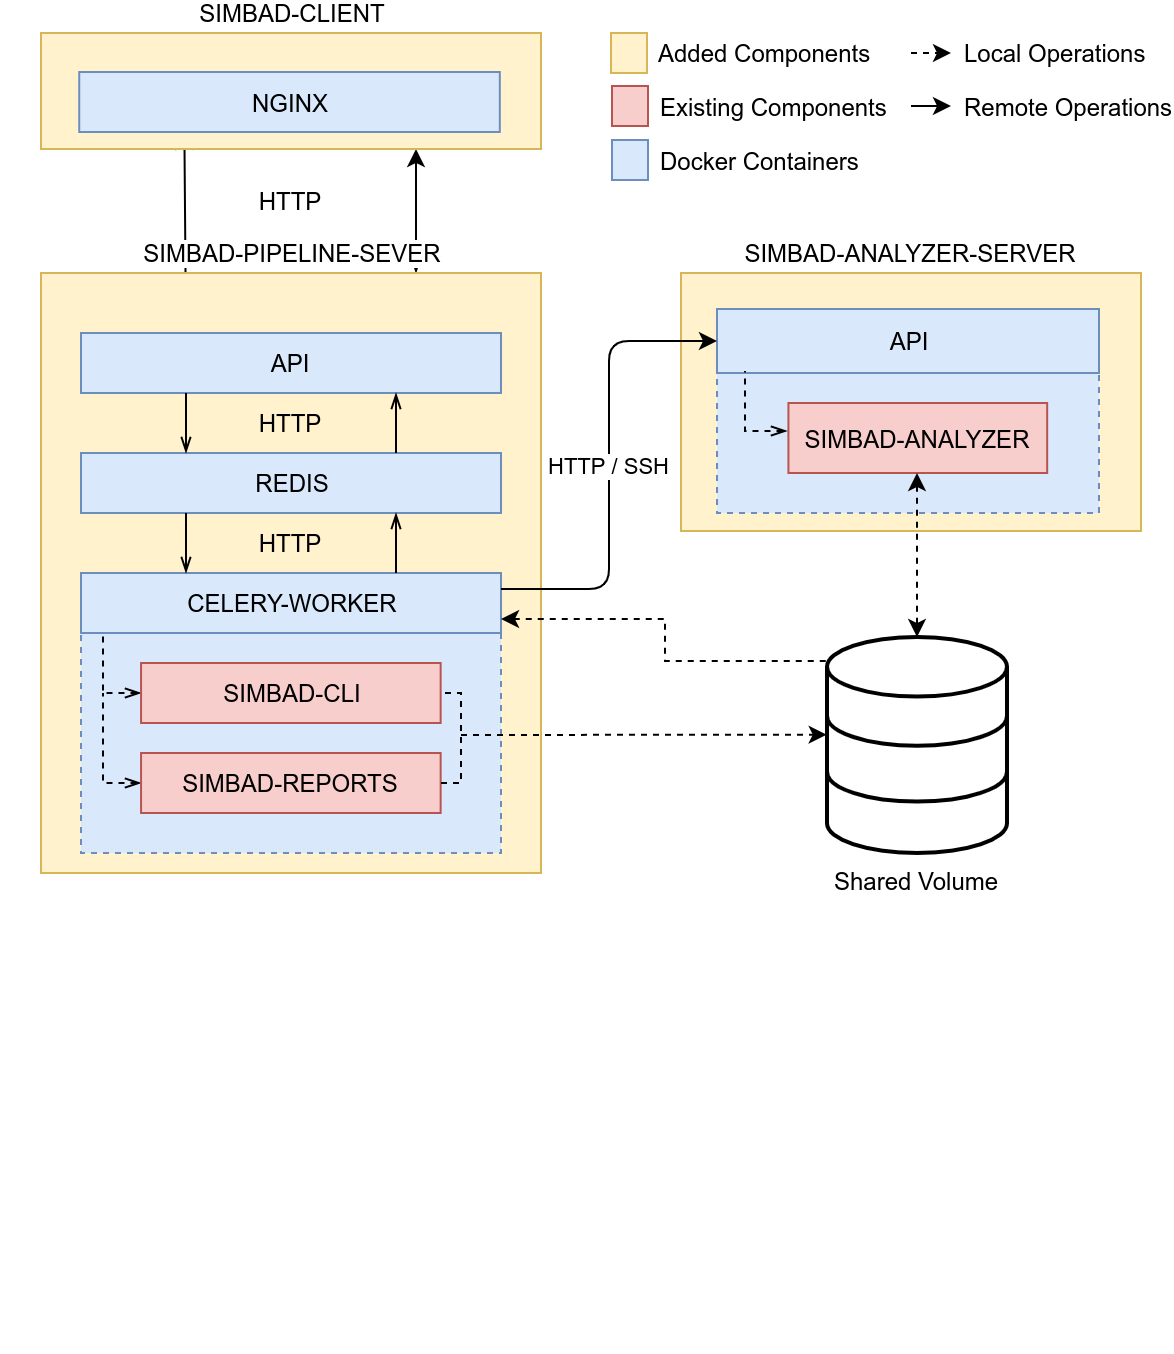
\includegraphics[width=0.9\linewidth]{diagrams/docker.png}
	\caption{Diagram of docker-compose containers}
	\label{fig:docker-containers}
\end{figure}
When simulation systems grows in a decoupled way, the number of docker container to manage also grows. To aid managing these containers, \textit{Docker Compose} was used. This tool can be used to define and manage application consisting of several components, placed on separate docker containers. The definition of application is placed in single \textit{docker-compose.yml} file. One can define services, shared volumes and networks in this file, and then start whole application using \textit{docker-compose up} command.. Containers are build from images that can be defined using \textit{Dockerfiles} or downloaded from \textit{Docker Hub}. Additionally, the network and volume definitions also can be placed in this file. Developing such system causes a need for two separate \textit{docker-compose} files, one for the developer, that builds docker images from source, and one for use, that pulls prebuild images from \textit{Docker Hub}. The docker-compose file that defines all of the simulation components using prebuild images is depicted on the listing \ref{list:docker-compose}. 
\begin{lstlisting}[label=list:docker-compose,caption=prod-docker-compose.yml file, basicstyle=\footnotesize\ttfamily, numbers=left, escapechar=|]
version: '3.4'
services:
  client:
    image: jsokolowski/simbad-client
    container_name: simbad-client
    ports:
      - "8080:80"
    volumes:
      - ./nginx.conf:/etc/nginx/nginx.conf
  pipeline:
    image: jsokolowski/simbad-pipeline-server |\label{line:sp}|
    container_name: simbad-pipeline-server
    command: python entrypoint_api.py --port 8081 --debug
    env_file:
      - ./docker.env
    ports:
      - "8081:8081"
    volumes:
      - ../data:/usr/data
  worker:
    image: jsokolowski/simbad-pipeline-worker
    container_name: celery-worker
    links:
      - analyzer-server
    command: celery worker -A entrypoint_celery.celery --loglevel=info
    env_file:
      - ./docker.env
    volumes:
      - ../data:/usr/data
  analyzer-server:  |\label{line:analyzer-server}|
    image: jsokolowski/simbad-analyzer-server
    container_name: simbad-analyzer-server
    command: python3 app.py --port 5000 --debug
    env_file:
      - ./docker.env
    volumes:
      - ../data:/usr/data
      - ./log4j.properties:/opt/spark-2.4.3-bin-hadoop2.7/conf/log4j.properties
    ports:
      - "5000:5000"
      - "4040:4040"
  redis:
    image: redis:alpine
    container_name: redis
    ports:
      - "6379:6379"
\end{lstlisting}
All of the simulation component containers are defined under the \textit{services} key, for example, \textit{analyzer-server} key visible on the line \ref{line:analyzer-server} of listing \textit{docker-compose} defines configuration of \textit{SAS} component. The \textit{image} key, under the \textit{analyzer-server}, specifies from where to pull the prebuild image from. The \textit{command} key specifies what command needs to be executed after container is started. The \textit{env\_file} key specified the path to file with environmental variables, that need to be set inside of container \textit{OS}. This file is also primary method of configuring the system and will be described in more detail in section \ref{appendix:configuration}. Shared volumes and files that need to be placed inside container can be defined using the \textit{volumes} key. First entry under that key is a shared volume, where the simulation files will reside. The \textit{"../data:/usr/data"} syntax, means that the local data folder will be mounted as \textit{/usr/data} folder inside of the container. The \textit{"value:value"} syntax in general can be interpreted as \textit{"HOST:CONTAINER"}. Similiary, second entry under this key copies local configuration file for \textit{log4j}, that is used to configure logging in \textit{ApacheSpark}. The last key is ports which is used to define which ports need to be exposed in container. The syntax \textit{"5000:5000"} means that the through port 5000 on \textit{Docker} host, it is possible to access port 5000 on \textit{Docker} container. Port 5000 on this container exposes the  \textit{SAS} \textit{API} and port 4000 is used to access \textit{SparkUI} dashboard.
Using the development version of the \textit{docker-compse.yml} file and few \textit{Docker Compose} commands, developer can easily make changes to system component, build the images from source, and publish them on \textit{Docker Hub}.
\section{System Configuration}
Two main sources of configuration are the \textit{docker-compose.yaml} files and \textit{docker.env} files. Form the compose files it is possible to specify ports and paths to data. The \textit{docker.env} file contains the definition of environment variables that will be set in every container it is passed to. In those files, there are more advanced settings, mostly for power users, such as which executor will run which task, the updates polling period, or external drives to be mounted via \textit{SSHFS}.
\subsection{Remote host}
To enable running components on separate machines, docker configuration most be modified. Example setup for such configuration could be \textit{SimBaD-Analyzer-Server} running on one  machine, and all other components running on the other.
For the sake of example, those two machines will be on the same network, the \textit{SAS} at 192.168.0.32 and the rest at 192.168.0.31. First step to enable that, is to extract the \textit{SAS} container to a separate docker compose file, visible on the listing \ref{list:docker-split}. The entry under the \textit{analyzer-server} key in original \textit{prod-docker-compse.yml} file should be removed, to prevent running redundant containers.
\begin{lstlisting}[label=list:docker-split,caption= docker-compose file for standalone \textit{SimBaD-Analyzer-Server}, basicstyle=\footnotesize\ttfamily, numbers=left, escapechar=|, numbers=left]
version: '3.4'
services:
  analyzer-server:
    image: jsokolowski/simbad-analyzer-server
    container_name: simbad-analyzer-server
    command: python3 app.py --port 5000 --debug
    env_file:
      - ./docker.env
    volumes:
      - sshfs:/usr/data
      - ./log4j.properties:/opt/spark-2.4.3-bin-hadoop2.7/conf/log4j.properties
    ports:
      - "5000:5000"
      - "4040:4040"
    network_mode:
      host
volumes:
    sshfs:
      name: sshfs
      driver: vieux/sshfs:latest
      driver_opts:
        sshcmd: "user@192.168.0.31:/home/user/simbad/data"
        password: "password"
\end{lstlisting}
The network mode is set to host, to make the container available from outside. It's worth noting, that this option works only on docker for \textit{GNU\textbackslash Linux}. Additionally to make the filesystem available to both machines, the \textit{SAS} must mount the filesystem of other machine, at the same mountpoint. This is done through \textit{SSHFS} \textit{Docker} extension. First, in the root volume key, the \textit{SSHFS} volume is defined, and then, it is mounted in the volume key under \textit{analyzer-server}. Second file that needs to be edited is the \textit{docker.env} file. In this file the address and port to \textit{SAS} must be set, and the \textit{TaskExecutor} for \textit{SimBaD-Analyzer} must be set to \textit{HTTP}. Fragment of such env file can be seen on the listing \ref{list:docker-split-env}. To start the system, user would need to enter docker-compose up on both machines.
\begin{lstlisting}[label=list:docker-split-env,caption=prod-docker-compose.yaml file, basicstyle=\footnotesize\ttfamily, numbers=left, escapechar=|]
...
SIMBAD_ANALYZER_HOST="192.168.0.32"
SIMBAD_ANALYZER_PORT="5000"
SIMBAD_ANALYZER_EXECUTOR=HTTP
...
\end{lstlisting}
